\documentclass[11pt]{article}
\usepackage{amsmath, amssymb, array}
\pagestyle{plain}

\textwidth=6.5in
\hoffset-1in
\textheight=9in
\voffset-1in

\usepackage{enumitem}
\usepackage{pgfplots}
\usepackage{graphicx}
\usepackage{lipsum}
\usepackage{stfloats}
\usepackage{multicol}
\setlength{\columnsep}{1cm}




\begin{document}


\noindent MATH 1113   \hfill 3.1 - Inverse Functions\\



\noindent \textbf{Topics:}  one-to-one functions, inverse functions, domain and range of inverse functions\\

\noindent \textbf{Student Learning Outcomes:}
\begin{enumerate}
\item Students will be able to determine if a function is one-to-one algebraically and graphically.
\item Students will be able to determine the inverse of a function.
\item Students will be able to determine the domain and range of an inverse function.
\end{enumerate}

\hrule 
\vspace{5mm}
\section{Identify One-to-One Functions}


\noindent \begin{tabular}{ | l  |} \hline
\noindent \underline{Horizontal Line Test.} A function is one-to-one if every horizontal line intersects \\ the graph of $f$ at most once. Otherwise the function is not one-to-one. \\  \hline
\end{tabular} 

\begin{enumerate}
\item Determine whether the graph is the graph of a one-to-one function.

 \begin{tabular}{c c }
\scalebox{0.7}{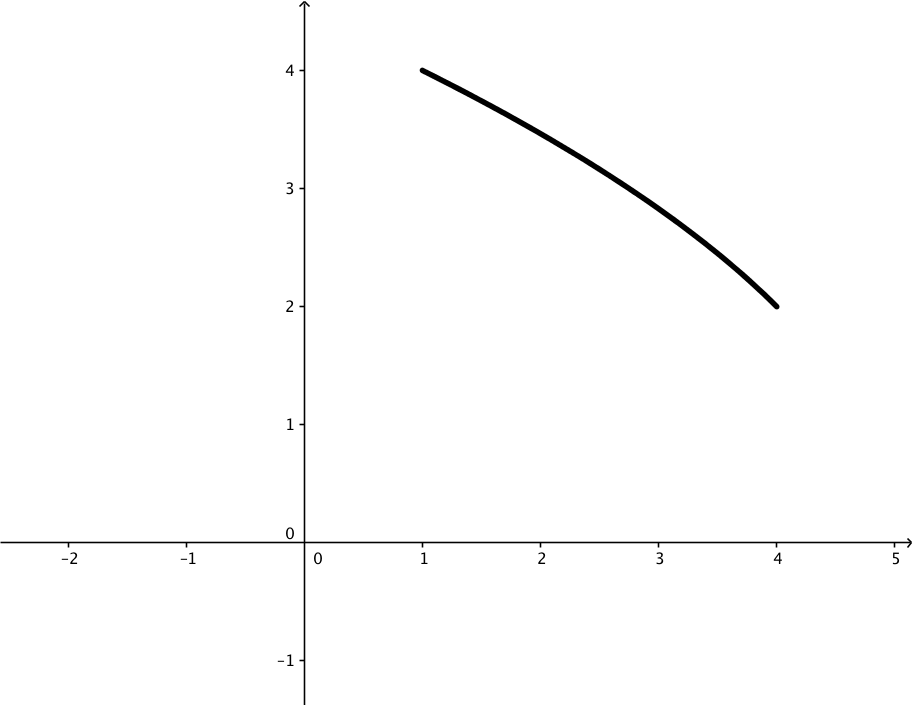
\includegraphics{oneone2}} &   \scalebox{0.7}{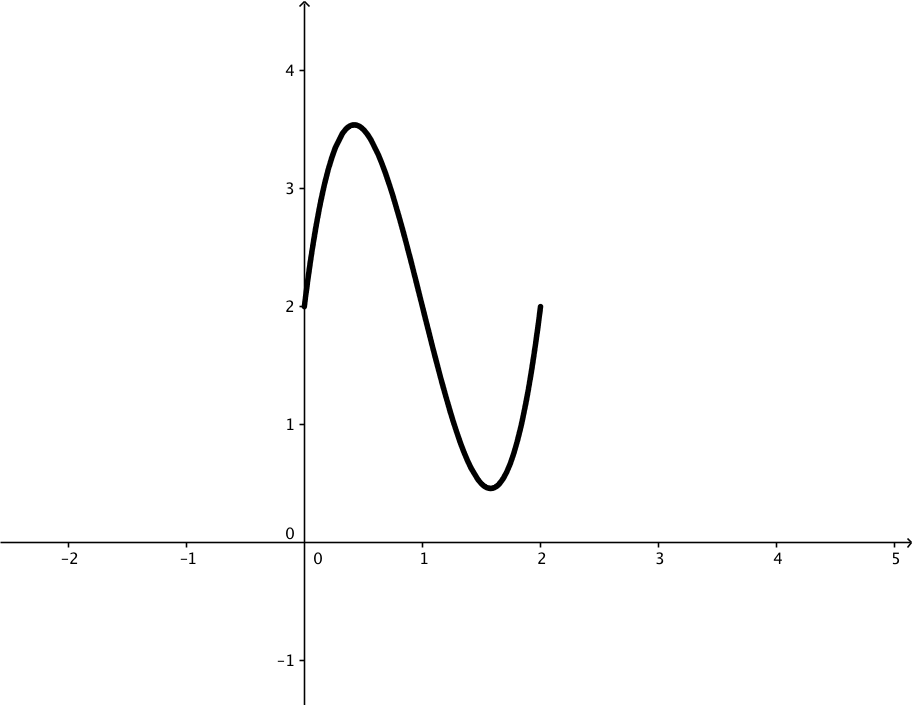
\includegraphics{oneone1}}  
\end{tabular} 

\item Determine whether the following functions are one-to-one.
\begin{enumerate}
\item $f=\{(1,4), (2,3), (-2,3)\}$\\[.5in]

\item $f(x) = \sqrt{5x}$
\vfill
\item $f(x) = x^2$
\end{enumerate}
\vfill


\newpage


\section{Determine Whether Two Functions are Inverses}


\noindent \begin{tabular}{ | l  |} \hline
\noindent \underline{Theorem on Inverse Functions.} Let $f$ be a one-to-one function with domain $D$ and  \\ range $R$. If $g$ is a function with domain $R$ and range $D$, then $g$ is the inverse \\ function of $f$ precisely when both of the following conditions hold:   \\ 
$ \star$ \quad $g(f(x))=x$ for every $x$ in $D$, and \\
$ \star$ \quad $f(g(y))=y$ for every $y$ in $R$.\\ \hline
\end{tabular} 

\noindent \textbf{Notation:}  "f inverse" is typically written as $f^{-1}$. It is important to note that $f^{-1}$ does NOT mean the same thing as $\dfrac{1}{f}$.


\item Let $f(x) = x^2+4, \quad x \geq 0$, and let $g(x) = \sqrt{x-4}, \quad x \geq 4 $

\begin{enumerate}
\item Use the theorem on inverse functions to determine whether $f$ and $g$ are inverses.  \\[2in]
\item Sketch the graphs of $f$ and $g$ on the same coordinate axes.

\scalebox{0.5}{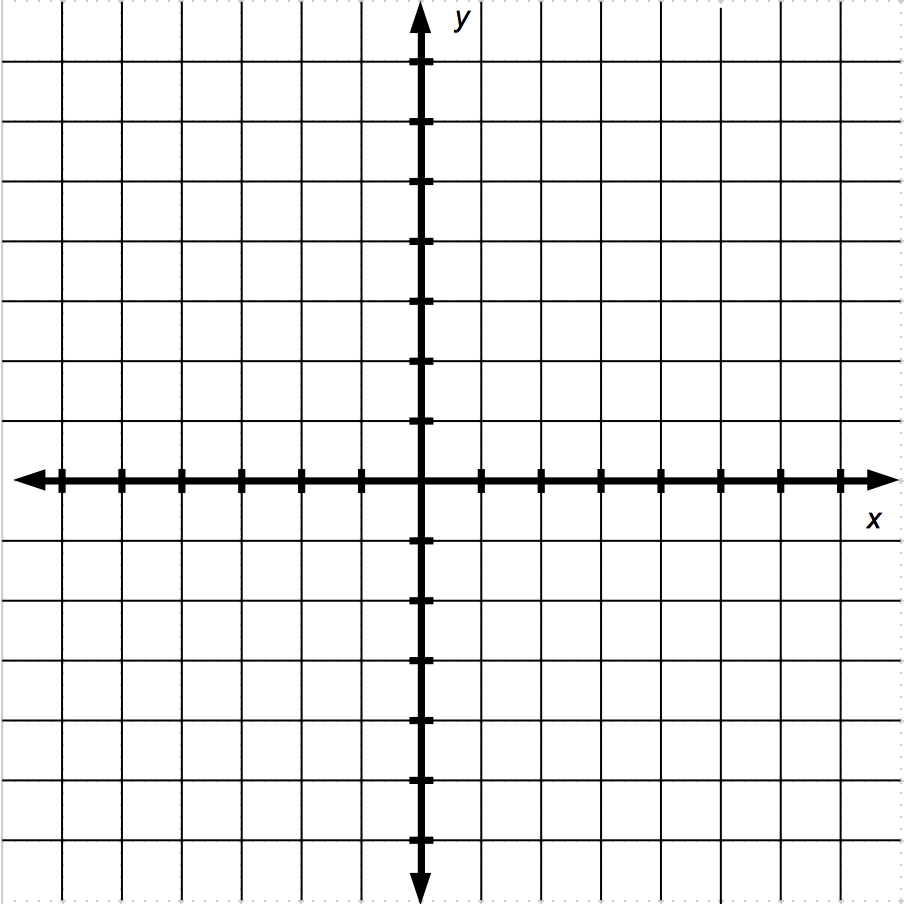
\includegraphics{bigaxes}}

\end{enumerate}


\newpage



\section{Find the Inverse of a Function}

\noindent \begin{tabular}{ | l  |} \hline
\noindent \underline{Guidelines for Finding Inverse Functions.} \\
Assuming that $f$ is a one-to-one function, and that the algebra is do-able, you can find $f^{-1}$ \\ using the following procedure: \\
1. Solve the equation $y=f(x)$ for $x$ in terms of $y$. You now have $x = f^{-1}(y)$. \\
2. Replace $x$ with $y$ and solve for $y$. This is your inverse function, replace $y$ with $f^{-1}(x)$. \\ 
3. Check your work (if time permits): check that $f^{-1}(f(x))=x$ whenever $x$ is in the domain\\ of $f$, and $f(f^{-1}(x))=x$ whenever $x$ is in the domain of $f^{-1}$. \\ \hline
\end{tabular} 


 
 \item Find the inverse function of $f(x) = 4 + 3x$. \\[1.2in]
 
 
 \vfill
 
  
\item Use the table for the one-to-one function $f(x)$ to compute each expression.\\[.2in]
\begin{tabular}{| c |  c | c | c | c | c | }
\hline x & 2 & 3&7 &6 & 15\\ \hline
f(x) &-1 &5 &4 &2 & 3\\ \hline
\end{tabular} 
\\
\begin{enumerate}
\item $f^{-1} (5)$ \\ \\
\item $f^{-1} (-1)$ \\ \\
\item $f^{-1} (2)$ \\ \\

\end{enumerate}




\end{enumerate}

\noindent \textbf{Student Learning Outcomes Check}

\begin{enumerate}
\item Can you determine if a function is one-to-one algebraically and graphically?
\item Are you able to determine the inverse of a function?
\item Can you determine the domain and range of an inverse function?

\end{enumerate}

\noindent \textbf{If any of your answers were no, please ask about these topics in class.}













\end{document}